\section{Architecture}
\label{section:architecture}

In Figure~\ref{fig:arch} we present the high-level architecture of the demo network 
and some details about interaction of the billing system with the Radius server
and frontend application. The presented architecture does not however describe
the interaction with the banks and other payment systems. 

\begin{figure}[!h]
	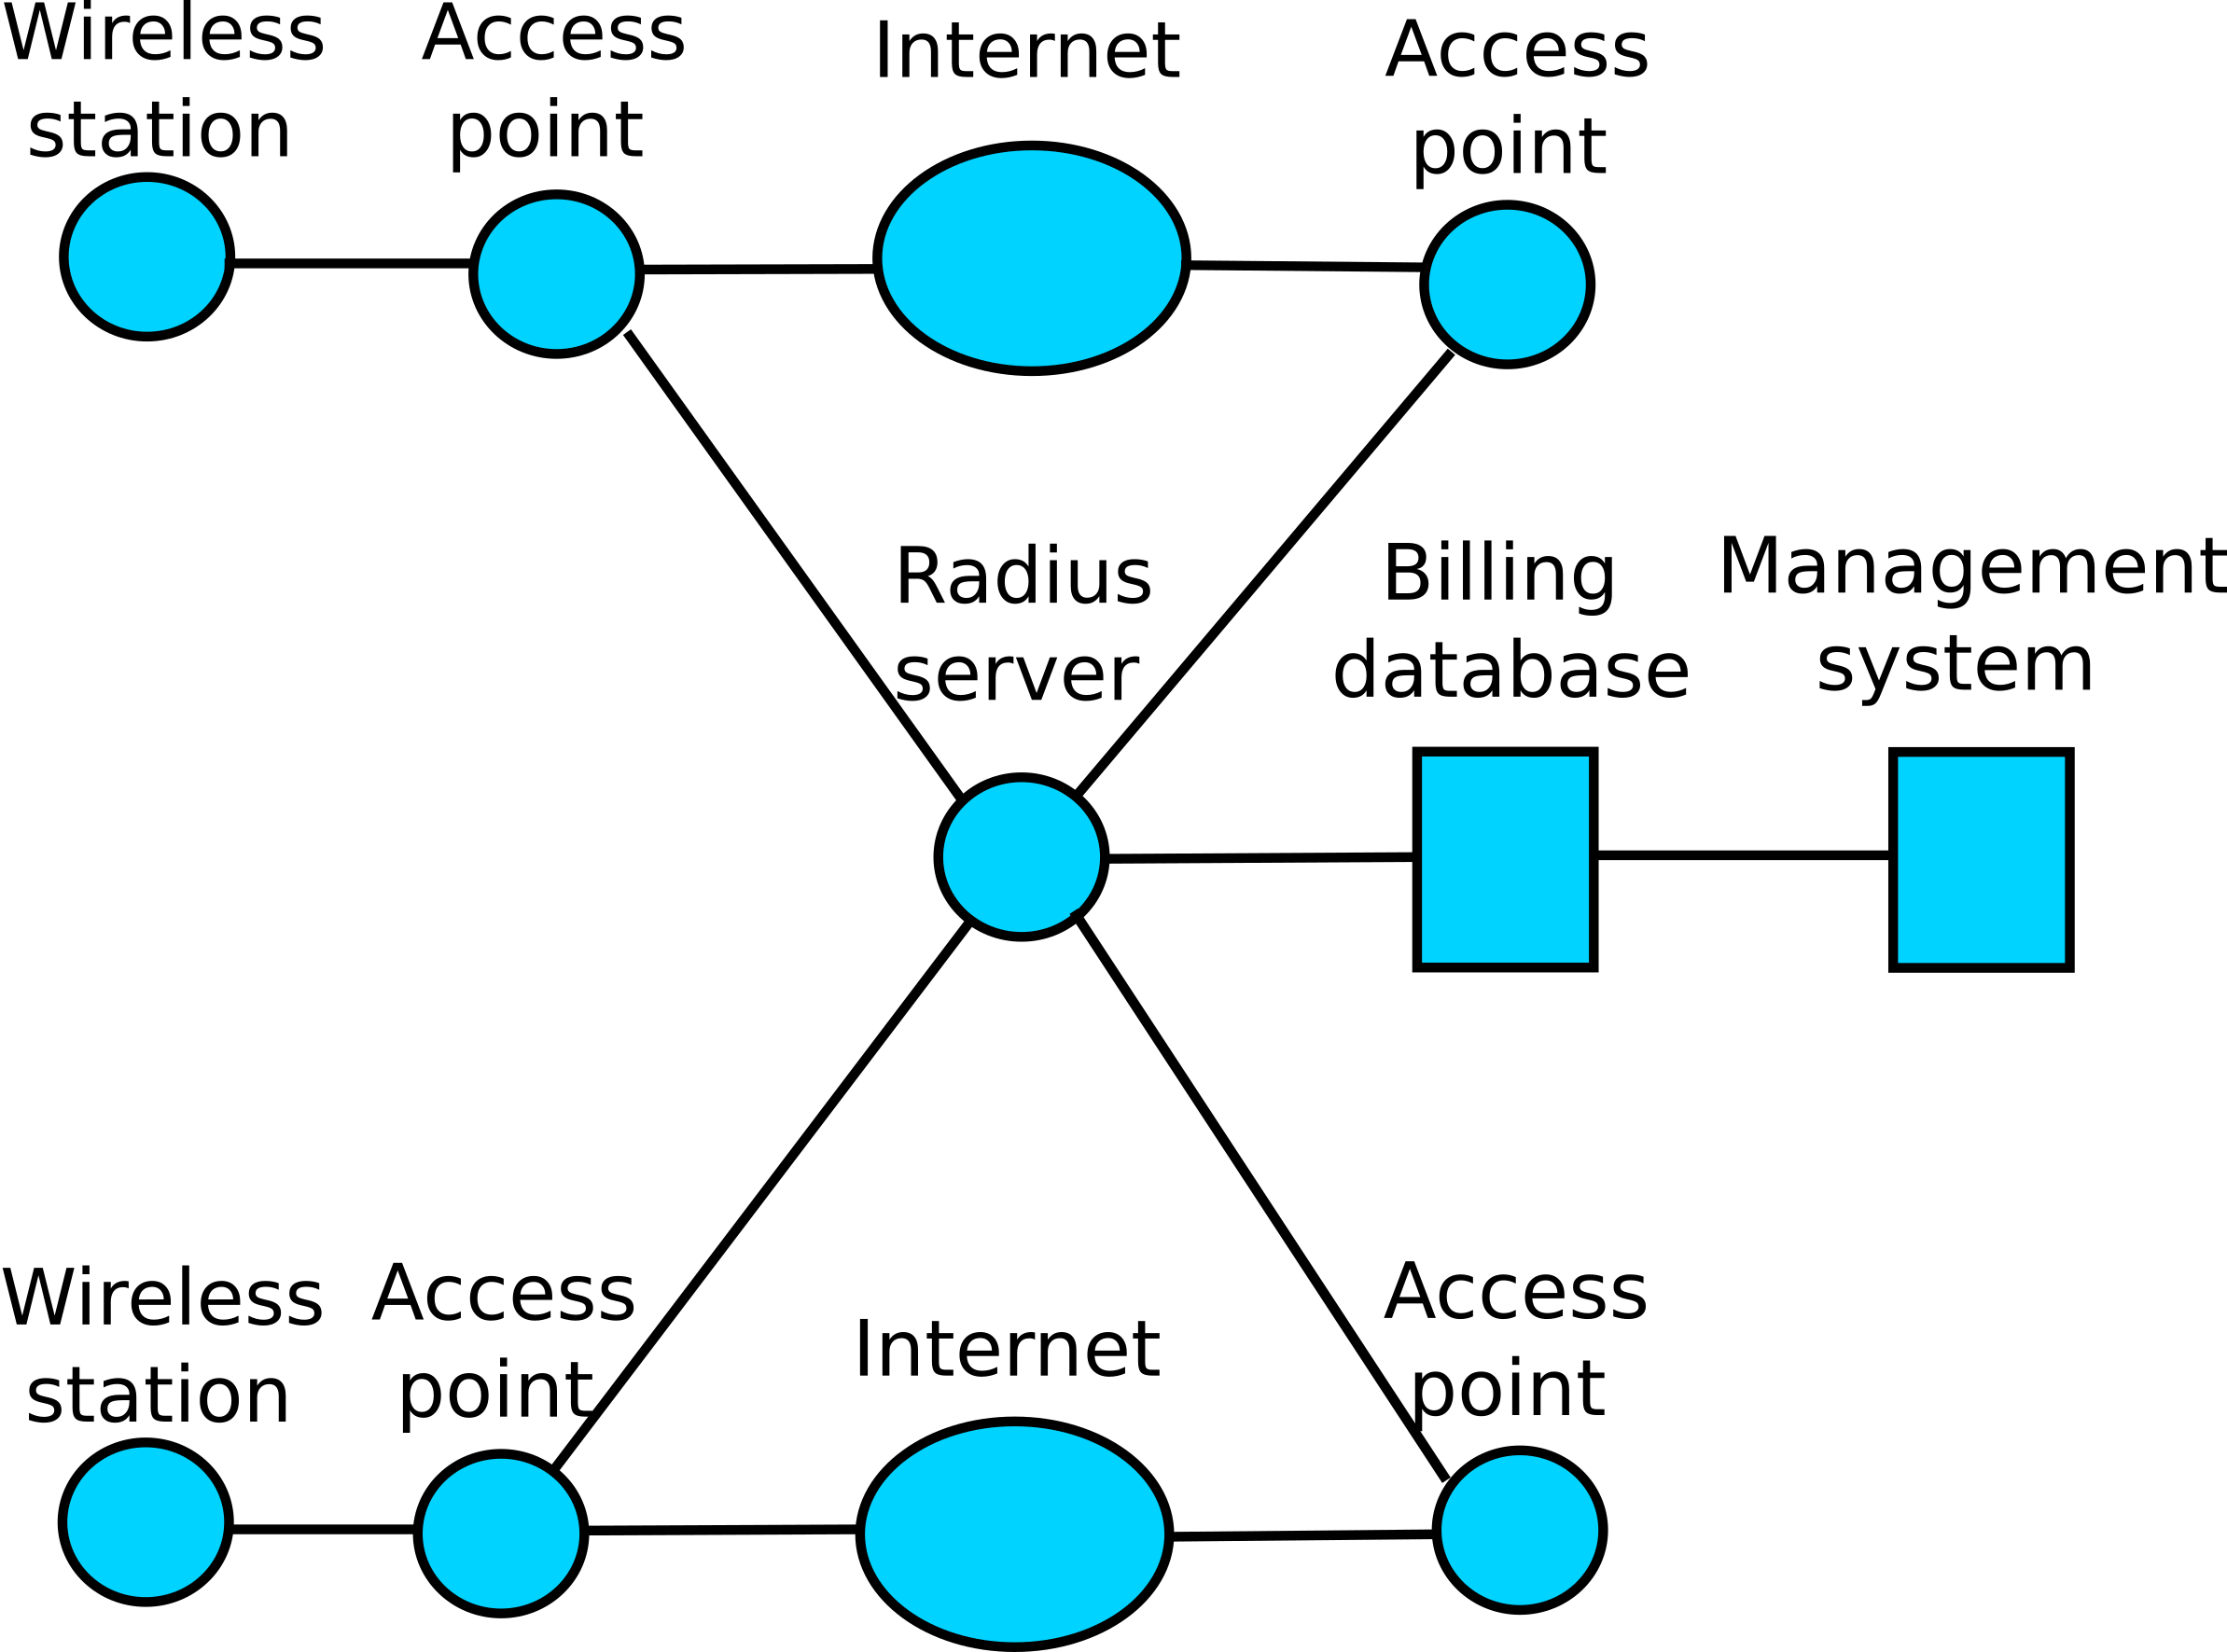
\includegraphics[width=0.5\textwidth]{graphics/arch.png}
	\caption{High-level architecture of the Intranet and billing system}
	\label{fig:arch}
\end{figure}

\section{Implementation}

We have opted to use our own custom implementation of a RADIUS server. 
Thus, using the following RFCs - RFC 2865 (RADIUS), RFC 5281 (EAP TTLS Authentication Protocol), 
RFC 2866 (RADIUS accounting), RFC 2869 (RADIUS Extensions), RFC 5246 (The Transport Layer 
Security (TLS) Protocol Version 1.2) - we have implemented basic RADIUS server
\footnote{The source code is available online at 
\url{https://github.com/dmitriykuptsov/radwi/tree/master/radius}}. Our implementation
comprises roughly $6K$ LOC and has minimal support for TLS server version 1.2 (we implemented 
support for only two cipher suits (i) TLS RSA with AES 256 in CBC mode for encryption and SHA 256 for 
hashing; (ii) TLS RSA with AES 128 in CBC mode for encryption and SHA 256 for 
hashing). 

\section{Configuration}

Our first step was related to configuration of MikroTik router. First, we have
created bridge interface and included WLAN1 and Ethernet ports in it. Then,
we have configured wireless adapter: (i) we have configured security profile (WPA-2 
Enterprise) and (ii) we have configured WLAN1 interface to operate in wireless access 
point mode. Finally, we have configured the RADIUS client on MikroTik with the 
following command.

\begin{verbatim}
radius add 
protocol=udp 
secret="highentropysecret" 
address=192.168.0.105 
service=wireless 
accounting-port=1813 
disabled=no
\end{verbatim}

Beacause decryption of pre-master secret takes more than one second (on the Raspberry PI), 
we had to increase the RADIUS timeout to two seconds, otherwise the 
RADIUS client was closing socket too early and kernel was sending 
\texttt{ICMP destination port unreachable} during the handshake.

We then configured our custom implementation of RADIUS server. Basically the only configuration that 
was required was related to generation of x509 certificate. We have accomplished this using \texttt{openssl} tool:

\begin{verbatim}
openssl req -newkey rsa:8192 
-nodes -keyout key.pem 
-x509 -days 365 
-out certificate.pem
\end{verbatim}

We have noticed that if the user does not specify the Certificate Authority's (CA) certificate, 
no alert is generated on Android phone signalizing that the certificate is self-signed.
